\documentclass{article}
\usepackage[utf8]{inputenc}
\usepackage{amsmath}
\usepackage[english]{babel} 
\usepackage{amssymb}
\usepackage{amsmath}
\usepackage{txfonts}
\usepackage{mathdots}
\usepackage[classicReIm]{kpfonts}
\usepackage{graphicx}
\usepackage{pgfplots}
\pgfplotsset{width=11cm,compat=1.16}
\graphicspath{ {./images/} }

\title{hw1}
\date{October 2020}

\begin{document}

\maketitle

\section{.}

eigenvalues of A=$\:\begin{pmatrix}2&0&0\\ \:1&2&1\\ \:-1&0&1\end{pmatrix}$

$\\det(A-\lambda *I)=\begin{vmatrix}
1-\lambda & -3 & 3 \\
3 & -5-\lambda & 3 \\
6 & -6 & 4-\lambda
\end{vmatrix}$

$\\=(-\lambda+1)*(-\lambda-5)*(-\lambda+4)+(-3)*3*6+3*3*(-6)-6*(-\lambda-5)*3-(-6)*3*(-\lambda+1)-(-\lambda+4)*3*(-3)=-\lambda^3+12*\lambda+16=-(\lambda+2)*(\lambda^2-2*\lambda-8)=-(\lambda+2)*(\lambda+2)*(\lambda-4) $

$ \lambda_1=-2,\lambda_2=4$\\
For every value we find its own vectors:\\
$\lambda_1=-2\\
A-\lambda_1*I=\left(\begin{matrix}
3 & -3 & 3 \\
3 & -3 & 3 \\
6 & -6 & 6
\end{matrix}\right)\xrightarrow{Line_2=Line_2 - Line_1}
\left(\begin{matrix}
3 & -3 & 3  \\
0 & 0 & 0  \\
6 & -6 & 6
\end{matrix}\right)\xrightarrow{Line_3=Line_3 - 2*Line_3}
\left(\begin{matrix}
3 & -3 & 3  \\
0 & 0 & 0  \\
0 & -0 & 0
\end{matrix}\right)$

for $(A-\lambda_1*I)X=0=>X=
\left(\begin{matrix}
x_2-x_3 \\
x_2 \\
x_3
\end{matrix}\right)$
\\The solution set:$\{x_2\left(\begin{matrix}1 \\ 1 \\ 0\end{matrix}\right)
                  x_3\left(\begin{matrix}-1 \\ 0 \\ 1\end{matrix}\right)
                  \}\\$
Let $x_2=1, x_3=0, v_1=\left(\begin{matrix}1 \\ 1 \\ 0\end{matrix}\right)$
Let $x_2=0, x_3=1, v_2=\left(\begin{matrix}-1 \\ 0 \\ 1\end{matrix}\right)\\$

$\lambda_2=4\\
A-\lambda_2*I=\left(\begin{matrix}
-3 & -3 & 3 \\
3 & -9 & 3 \\
6 & -6 & 0
\end{matrix}\right)\xrightarrow{Line_2=Line_2 + Line_1}
\left(\begin{matrix}
-3 & -3 & 3  \\
0 & -12 & 6  \\
6 & -6 & 0
\end{matrix}\right)\xrightarrow{Line_3=Line_3 + 2*Line_1}
\left(\begin{matrix}
-3 & -3 & 3  \\
0 & -12 & 6  \\
0 & -12 & 6
\end{matrix}\right)\xrightarrow{Line_3=Line_3 -Line_2}
\left(\begin{matrix}
-3 & -3 & 3  \\
0 & -12 & 6  \\
0 & 0 & 0\end{matrix}\right)\xrightarrow{Line_1/-3,Line_2/-12}
\left(\begin{matrix}
1 & 1 & -1  \\
0 & 1 & \frac{-1}{2} \\
0 & 0 & 0 
\end{matrix}\right)\\ \xrightarrow{Line_1=Line_1 -Line_2}
\left(\begin{matrix}
1 & 0 & \frac{-1}{2} \\
0 & 1 & \frac{-1}{2} \\
0 & 0 & 0
\end{matrix}\right)\\
$
So $x_2=1/2*x_3$ and $x_1=1/2*x_3 =>$
for $(A-\lambda_2*I)X=0=>X=\left(\begin{matrix}
\frac{1}{2}*x_3 \\
\frac{1}{2}*x_3 \\
x_3
\end{matrix}\right)$

The solution set:$\{x_3\left(\begin{matrix}1/2 \\ 1/2 \\                     1\end{matrix}\right)\\$
Let $x_3=1, v_3=\left(\begin{matrix}1/2 \\ 1/2 \\ 1\end{matrix}\right)$



\section{.}

\pgfplotsset{width=15cm,compat=1.16} 

\begin{tikzpicture} \begin{axis}[
    title={$x^3-4x\,-y^2$},
    enlarge x limits,
    view={0}{90},
    xlabel=$x$, ylabel=$y$,
    big,
]
\addplot3[domain=-10:10,
        domain y=-10:10,
        contour gnuplot={levels={-10,10},labels=false},
        thick,samples=50,samples y=50,
    ] {x^3-(4*x)-y^2};
\end{axis}

\end{tikzpicture}
\\
D = fxx(a,b) fyy(a,b) - $fxy^2(a,b)$\\
a) If D $>$ 0 and fxx (a,b) $>$ 0, then f has a relative minimum at (a,b).\\
b) If D $>$ 0 and fxx (a,b) $<$ 0, then f has a relative maximum at (a,b).\\
c) If D $<$ 0, then f has a saddle point at (a,b).\\
d) If D $=$ 0, then no conclusion can be drawn.\\
\\
for fx(x,y)=$3x^2$-4=fy(x,y)=2y=0 =$>$\\
y=0,x=2/$\sqrt[2]{3}$\\ \\
fxx(x,y)=6x, fyy(x,y)=2 ,fxy(x,y)=0\\
D=fxx(2,0)fyy(2,0) - $fxy^2(2,0)$=12*2 - 0=24$>$0 also fxx(2,0)$>$0 so f has a local minimum at the point (2,0,f(2,0)) = (2,0,0)
\section{.}
\begin{figure}[htp]
    \centering
    \includegraphics[width=10cm]{photos/Scan_20201108.png}
    \caption{}
    \label{}
\end{figure}
\section{.}

A.\\
\begin{figure}[htp]
    \centering
    \includegraphics[width=6cm]{photos/1.png}
    \caption{The function becomes periodic with T decreasing,$u=2,x_0=0.3$}
    \label{fig:1}
\end{figure}
\\
\begin{figure}[htp]
    \centering
    \includegraphics[width=6cm]{photos/2.png}
    \caption{The function becomes chaotic $u=3,x_0=0.3$}
    \label{fig:2}
\end{figure}
\\
\begin{figure}[htp]
    \centering
    \includegraphics[width=6cm]{photos/3.png}
    \caption{The function becomes chaotic by going to infinity $u=4,x_0=0.3$}
    \label{fig:3}
\end{figure}
\\
\begin{figure}[htp]
    \centering
    \includegraphics[width=6cm]{photos/1b.png}
    \caption{The function becomes chaotic $u=3,x_0=0.3$}
    \label{fig:1b}
\end{figure}
\\
\begin{figure}[htp]
    \centering
    \includegraphics[width=6cm]{photos/2b.png}
    \caption{The function becomes chaotic by going to infinity, $u=3,x_0=1.1$}
    \label{fig:2b}
\end{figure}
\\
\section{.}
a)\\ 
S'=$\tfrac{\mathrm{d}}{\mathrm{d}x}\left[\dfrac{1}{\mathrm{e}^{-x}+1}\right]
=-\dfrac{\mathrm{e}^{-x}}{\left(\mathrm{e}^{-x}+1\right)^2}=-\dfrac{(\mathrm{e}^{-x}+1)-1}{\left(\mathrm{e}^{-x}+1\right)^2}=-\dfrac{1}{\mathrm{e}^{-x}+1}+\dfrac{1}{\left(\mathrm{e}^{-x}+1\right)^2}=S(S-1)$\\
b)\\
S=$\tfrac{\mathrm{d}}{\mathrm{d}x}\left[\tanh\left(x\right)\right]=\dfrac{1}{\cosh^2\left(x\right)}=\dfrac{\cosh^2\left(x\right)-\sinh^2\left(x\right)}{\cosh^2\left(x\right)}=1-\tanh(x)=$1-S\\
c)\\
Set $S_a$ as S from subquestion a),\\
$S=x*S_a=>S'=S_a+x*S'_a=S_a+x(S_a(S_a-1))=S_a(1-x+xS_a)=\dfrac{S(1-x+S)}{x}$\\
d)\\
Set $S_b$ as S from subquestion b),\\
$S=x*S_b=>S'=S_b+x*S'_b=S_b+x(1-S_b^2)=S_b(1-x*S_b)+x=\dfrac{S(1-S)+x^2}{x}$


\section{.}
\[S(x)=\frac{1}{1+e^{-cx}},c>0=>\]
0$<S(x)<1$ for every value of x  
$1+e^{-cx}={1/S(x)}=>
e^{-cx}=1/S(x)-1=>$\[x=ln(\frac{S(x)}{-S(x)+1})/c\]

$
\tfrac{\mathrm{d}}{\mathrm{d}s}\left[\ln\left(\dfrac{s}{1-s}\right)\right]
=\dfrac{1-s}{s}\cdot\tfrac{\mathrm{d}}{\mathrm{d}s}\left[\dfrac{s}{1-s}\right]
=\dfrac{+s-s+1}{(1-s)s}=\dfrac{-1}{(s-1)s}>0 $
\\because 0$<s<1$ So x strictly increases with S
\\ \\$x=S^{-1}(S(x))=>\\dx/dx=d(S^{-1}(S(x)))/dx=>\\1=S^{-1}'(S(x))*S'(x)=>\\1/S'(x)=S^{-1}'(S(x))$
\\ Because S'(x)$>$0 ,$ S^{-1}'(S(x))>0$ so the “inverse function” x increases with S, if S’$>$0.

\section{.}
 S(x)=max(0,x)+a min(0,x),which for x$>$0=$>$ S(x)=x=$>$S'(x)=1,
 else S(x)=a*x=$>$S'(x)=a. 
 \begin{tikzpicture}
 \begin{axis}[
 title=Plot of S(x) and a equal to 0.01,
 xlabel={$x$},
 ylabel={$y$},
 width=9cm,
 height=9cm
 ]
 \addplot[blue]table{
 x      y
 -10    -10
 0      0
 10     0.1
 };
 \end{axis}
 \end{tikzpicture}
 \\
  \begin{tikzpicture}
 \begin{axis}[
 title=Plot of S(x) and a equal to 0.25,
 xlabel={$x$},
 ylabel={$y$},
 width=9cm,
 height=9cm
 ]
 \addplot[blue]table{
 x      y
 -10    -10
 0      0
 10     4
 };
 \end{axis}
 \end{tikzpicture}
\section{.}

\begin{tikzpicture}
\begin{axis}[
        xmin=-3, xmax=3, % x scale
        ymin=-2, ymax=0.5, % y scale
        legend entries={$n_1^1=pw_{1,1}^1 +b_1^1=-0.27*p-0.48$}
]
\addplot    {-0.27*x-0.48};
\end{axis}
\end{tikzpicture}
\\
\begin{tikzpicture}
\begin{axis}[
        xlabel=$x$,
        ylabel=$y$,
        xmin=-3 ,xmax=3,
        ymin=0, ymax=1, % y scale
        legend entries={$a_1^1=swish(n_1)=1/(1+e^{-\beta*n_1)}$}
]
\addplot    {1/(1+e^(0.27*x+0.48))};
\end{axis}
\end{tikzpicture}
\\
\begin{tikzpicture}
\begin{axis}[
        xmin=-3, xmax=3, % x scale
        ymin=-1.5, ymax=1.5, % y scale
        legend entries={$n_2^1=pw_{2,1}^1 +b_2^1=-0.41*p-0.13$}
]
\addplot    {-0.41*x-0.13};
\end{axis}
\end{tikzpicture}


\begin{tikzpicture}
\begin{axis}[
        xlabel=$x$,
        ylabel=$y$,
        xmin=-3 ,xmax=3,
        ymin=0, ymax=1, % y scale
        legend entries={$a_2^1=swish(n_2)=1/(1+e^{-\beta*n_2)}$}
]
\addplot    {1/(1+e^(0.41*x+0.13))};
\end{axis}
\end{tikzpicture}

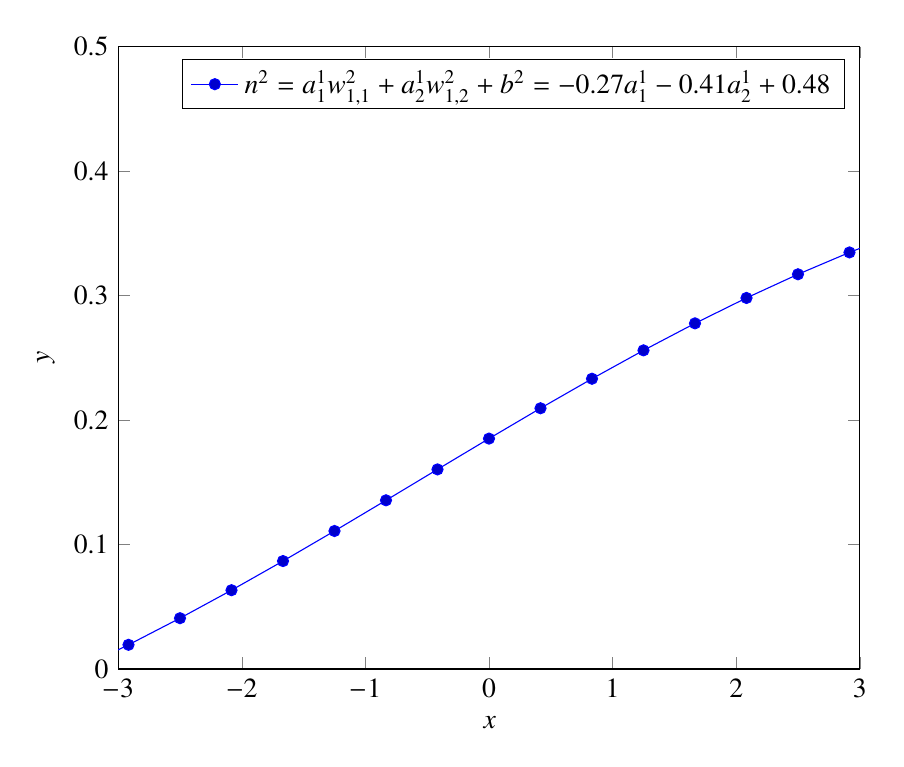
\begin{tikzpicture}
\begin{axis}[
        xlabel=$x$,
        ylabel=$y$,
        xmin=-3 ,xmax=3,
        ymin=0, ymax=0.5, % y scale
        legend entries={$n^2=a_1^1w_{1,1}^2 +a_2^1w_{1,2}^2+b^2=-0.27a_1^1-0.41a_2^1+0.48$}
]
\addplot    {-0.41/(1+e^(0.41*x+0.13))-0.27/(1+e^(0.27*x+0.48))+0.48};
\end{axis}
\end{tikzpicture}

\begin{tikzpicture}
\begin{axis}[
        xlabel=$x$,
        ylabel=$y$,
        xmin=-3 ,xmax=3,
        ymin=0, ymax=0.1, % y scale
        legend entries={$a_2=max{0,n^2}+min{0,n^2}=0.1n^2$}
]
\addplot    {-0.041/(1+e^(0.41*x+0.13))-0.027/(1+e^(0.27*x+0.48))+0.048};
\end{axis}
\end{tikzpicture}



\section{.}
a)\\
p = [[1,0],[1,-1],[0,-1],[0,1],[-1,0], [1,1]]\\
    t = [0,0,0,1,1,1]\\
    w = [0,0]\\
    b = 1\\

    while True:\\
        counter = 0\\
        for i in range(8):\\
            a = vector$_$mul(w,p[i]) + b\\
            #Calculate error\\
            e = t[i] - a\\
            if e == 0:\\
                counter += 1\\
            w[0] = w[0] + e*p[i][0]\\
            w[1] = w[1] + e*p[i][1]\\
            b = b + e\\
        if counter == 8:\\
            break\\

    print (f"Final weight: {w} and bias: {b}")\\

    for i in range(8):\\
        a = hardlim(vector$_$mul(w,p[i]) + b)\\
        print (f"P{i} is {a} and is supposed to be {t[i]}")\\
        
        \\\\Final weight: [-1, 2] and bias: -1

b)\\
\begin{figure}[htp]
    \centering
    \includegraphics[width=4cm]{photos/diagram.png}
    \caption{Diagram}
    \label{}
\end{figure}
\\c)\\
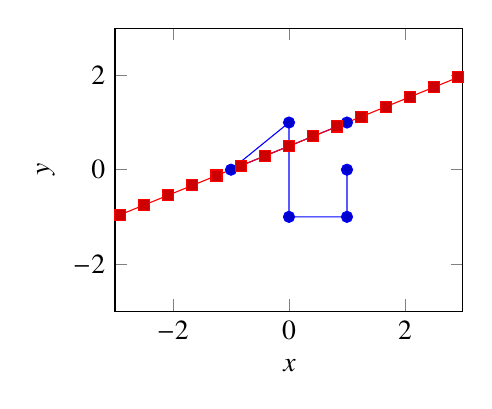
\begin{tikzpicture}
\begin{axis}[
        width=6cm,
        xlabel=$x$,
        ylabel=$y$,
        xmin=-3 ,xmax=3,
        ymin=-3, ymax=3, % y scale
]
\addplot coordinates {(1,0)(1,-1)(0,-1)(0,1)(-1,0)(1,1)};
    \addplot{x/2+1/2};
\end{axis}
\end{tikzpicture}
\\d)\\
By adding the vector[0 0] to Class I the network classifies it correctly\\
e)\\
The vector is already classified correctly,therefore there is no need for any change


\section{.}
\begin{figure}[htp]
    \centering
    \includegraphics[width=11cm]{photos/10.jpg}
    \caption{}
    \label{}
\end{figure}

\begin{figure}[htp]
    \centering
    \includegraphics[width=11cm]{photos/10_2.jpg}
    \caption{}
    \label{}
\end{figure}
\begin{tikzpicture} \begin{axis}[
    title={$1-1.1*x+0.1*y+0.825*x*x-0.25*x*y+1.2*y*y$},
    enlarge x limits,
    view={0}{90},
    xlabel=$x$, ylabel=$y$,
]
\addplot3[domain =-40:40,
        domain y=-10:10,
        contour gnuplot={levels={-10,10},labels=false},
        thick,samples=50,samples y=50,
    ] {1-1.1*x+0.1*y+0.825*x*x-0.25*x*y+1.2*y*y};
\end{axis}

\end{tikzpicture}
\newpage
\section{.}

The mean square error can be expressed as $F(X)=c-2X^{T} h+X^{T} RX$, and c, h and R can be calculated by:


 
\[c=E[t^{2} ]=0.75(1)^{2} +0.25(-1)^{2} =1\] 

\[\begin{array}{l} {h=E[tZ]=0.75(1)\left[\begin{array}{l} {1} \\ {1} \end{array}\right]+0.25(-1)\left[\begin{array}{l} {-1} \\ {-1} \end{array}\right]=\left[\begin{array}{l} {1} \\ {1} \end{array}\right]} \\ {R=E[ZZ^{T} ]=0.75\left[\begin{array}{l} {1} \\ {1} \end{array}\right]\left[\begin{array}{cc} {1} & {1} \end{array}\right]+0.25\left[\begin{array}{l} {-1} \\ {-1} \end{array}\right]\left[\begin{array}{cc} {-1} & {-1} \end{array}\right]=\left[\begin{array}{cc} {1} & {1} \\ {1} & {1} \end{array}\right]} \end{array}\] 


 so the mean square error performance index is

 
\[F(X)=1-2\left[\begin{array}{cc} {w_{1,1} } & {w_{1,2} } \end{array}\right]\left[\begin{array}{l} {1} \\ {1} \end{array}\right]+\left[\begin{array}{cc} {w_{1,1} } & {w_{1,2} } \end{array}\right]\left[\begin{array}{cc} {1} & {1} \\ {1} & {1} \end{array}\right]\left[\begin{array}{l} {w_{1,1} } \\ {w_{1,2} } \end{array}\right]\] 
          
\[=1-2(w_{1,1} +w_{1,2} )+(w_{1,1} +w_{1,2} )^{2} \] 


 

The eigen values and eigen vectors of Hessian matrix of F(x) is

  

 A=2*[1 1;1 1];

 [V,D] = eig (A)  

 

 V =

     0.7071    0.7071

    -0.7071    0.7071

 D =

          0         0

          0    4.0000  

 

  Since all the eigen values are non-negative, and one is zero, there's a weak minimum in this problem. The surface and contour plot of F(x) are shown in Fig.1 and Fig.2.

 

\begin{enumerate}
\item  The maximum stable learning rate will satisfy $\alpha <\frac{2}{\lambda _{\max } } =\frac{2}{4} =0.5$.
\end{enumerate}


\begin{enumerate}
\item  Take $\alpha =0.2$. After 40 iterations we got $w_{1,1} =0.5,w_{1,2} =0.5$ (W${}_{1}$ in the code), and the trajectory is shown in Fig.2 as dotted symols.
\end{enumerate}


 

 clear

 [X,Y] = meshgrid(-3 : .1 : 3);

 F = 1 - 2 * (X + Y) + (X + Y).$\boldsymbol{\mathrm{\wedge}}$2;
 surf(X,Y,F)
 figure;
 contour(X,Y,F)
 hold on;

 \%Initialize data

 P = [1 -1;1 -1];

 T = [1 -1];

 alfa = 0.2;

 W1 = [0;0];

 W2 = [1;1];

 for k = 1 : 2

\qquad    if (k == 1)

\qquad \qquad       W = W1;

\qquad    else

\qquad \qquad       W = W2;

\qquad    end

    plot(W(1), W\eqref{GrindEQ__2_},'r*')

    text(-0.3,-0.3,'W\_0 =(0,0)');

    text(1,1.2,'W\_0 =(1,1)');

 for step = 1 : 20

\qquad    for i = 1 : 2

\qquad \qquad       a = purelin(W' * P(:,i));

\qquad \qquad       e = T(i) - a;

\qquad \qquad       W = W + 2 * alfa * e * P(:,i);

\qquad \qquad          if (k == 1)

\qquad \qquad \qquad             plot(W(1), W\eqref{GrindEQ__2_},'k.')

\qquad \qquad \qquad             W1 = W;

\qquad \qquad          else 

\qquad \qquad \qquad             plot(W(1), W\eqref{GrindEQ__2_},'b+')

 \qquad \qquad \qquad            W2 = W;

\qquad \qquad          end

\qquad \qquad    end

\qquad end

 end

 W1

 W2

 hold off; 

 

 W1 =

\qquad     0.5000

\qquad     0.5000

 W2 =

\qquad     0.5000

\qquad     0.5000

\begin{figure}[htp]
    \centering
    \includegraphics[width=6cm]{photos/mean_error.png}
    \caption{Mean square error}
    \label{}
\end{figure}
\begin{figure}[htp]
    \centering
    \includegraphics[width=6cm]{photos/pic2.png}
    \caption{Trajectory}
    \label{}
\end{figure}
\\
iv. For initial weights [1 1], after 40 iterations, we got   (W2 in the code), and the trajectory is also shown in Fig.2 as "+" symols. And the decision boundary is given in Fig.3.
\\
P = [1 -1;1 -1];
W = [0.5 0.5];\\
figure;\\
plot(P(1,1),P(2,1),'r+');\\
hold on;\\
plot(P(1,2),P(2,2),'r+');\\

x = -2 : .1 : 2;\\
y =(-W(1)*x )/W(2);\\
plot(x,y);\\
axis([-2 2 -2 2]);\\

hold off;  \\
img3\\
e)\\
	From the figure above, we can see that LMS algorithm, unlike the perceptron learning rule, places the decision boundary as far from the patterns as possible.\\

Also, we see that for 2 different initial weights, the solution converges to the same value. However, if other arbitrary initial points are selected, we could get different solutions, since the performance index only has a weak minimum, i.e. the minimum is not unique. There's a line on which all the mean square error is minimum (zero). \\


     
\section{.}


\section{.}



\begin{tabular}{|c|c|c|c|c|c|c|}
    \hline
  p &  q & \lnot p & \lnot p \land q   & p \lor (\lnot p \land q )    & \lnot(p \lor (~p \land q )) & \lnot(p \lor (~p \land q )) \land q\\
    \hline
    0 & 0 & 1 & 1 & 0 & 1 & 1\\
    \hline
    0 & 0.5 & 1 & 1 & 0 & 1 & 1\\
    \hline
    0 & 1 & 1 & 1 & 0 & 1 & 1\\
    \hline
    0.5 & 0 & 0.5 & 0.5 & 0.5 & 0.5 & 0.5\\
    \hline
    0.5 & 0.5 & 0.5 & 0.5 & 0.5 & 0.5 & 0.5\\
    \hline
    0.5 & 1 & 0.5 & 1 & 0.5 & 0.5 & 1\\
    \hline
    1 & 0 & 0 & 0 & 0 & 1 & 1\\
    \hline
    1 & 0.5 & 0 & 0.5 & 0.5 & 0.5 & 0.5\\
    \hline
    1 & 1 & 0 & 1 & 1 & 0 & 1\\
    \hline
\end{tabular}
\medskip


\begin{tabular}{|c|c|c|c|c|c|c|}
$    \hline
  p &  q & \lnot p & \lnot p \land q   & p \lor (\lnot p \land q )    & \lnot(p \lor (~p \land q )) & \lnot(p \lor (~p \land q )) \land q\\
    \hline
    0 & 0 & 1 & 1 & 0 & 1 & 1\\
    \hline
    0 & 1 & 1 & 1 & 0 & 1 & 1\\
    \hline
    1 & 0 & 0 & 0 & 0 & 1 & 1\\
    \hline
    1 & 1 & 0 & 1 & 1 & 0 & 1\\
    \hline $
\end{tabular}
\medskip
If we use crisp logic over fuzzy the "(P(x) and (P(x)$->$ Q(x))) $->$ Q(x)" becomes tautology.

\section{.}

Dimitris and Fany go to park if it is a beautiful day and it is not too hot, or if it isn't raining.\\
With  Assuming that it is a beautiful day with 0.7 degree,it is hot with 0.3 degree and it is raining with 0.6 degree . We have:\\
$(0.7 degree \land \lnot 0.3  degree)  \lor \lnot0.6 degree  \\
(0.7 degree \land  0.7  degree)  \lor 0.4 degree \\
0.7  degree  \lor 0.4 degree  \\
0.7 degree \\
$
So  Dimitris and Fany will go to park with 0.7 degree \\

\end{document}
